% !TeX spellcheck = en_US
\documentclass[12pt]{report}
\usepackage{paccopsde}
	\makeindex
\begin{document}
	\title{Partial Stochastic Differential Equations}
	\author{Kotatsu}
	\date{\small BADIALE VAFFANCULOOOOOOOOOO}
	\maketitle
	\pagenumbering{Roman}
	\begin{preface}
		These are the notes of the Stochastic Processes course for the Academic Year 2025-2026 with Professors Toaldo and Badiale.\par
		I took these notes personally and I integrated the (many) unclear parts and passages using online resources and occasionally the fucking shitty books that this course has. \par
		I am not particularly enthusiast about this course but, as a person with no mathematical background from bachelor degree, I firmly believe in the necessity to understand what you are fucking doing and therefore I went out of my way to make these notes as understandable as possible for other wretched people that have not taken a single analysis exam in their whole life and now have to face integral equations. 
		
		GOD I HATE THIS UNIVERSITY
		\vskip1.2cm
		
		\hfill Kotatsu
		\vskip1.2cm
		Check the source code for this and other notes in my GitHub repo $\to$ \href{https://github.com/godblessourdeadkotatsu/lecture-notes-2024-25/tree/main/PSDE}{\faGithubSquare}
	\end{preface}
	\clearpage
	\tableofcontents
	\pagenumbering{arabic}
\chapter{The Itô integral}	
\section{Introduction}
Imagine we have a random phenomenon whose realization is 
\begin{equation*}
	\seqtm{X}.
\end{equation*}
Imagine the infinitesimal increment 
\begin{equation*}
	\seqtdt{X}.
\end{equation*}
This is proportional to the time integral
\begin{equation*}
	\seqtdt{X}=X_{t}=b\dt
\end{equation*}
which is just a deterministic quantity proportional to the time increment $\dt$. Now add a source of randomness like a noise \rv{} $Z$:
\begin{equation*}
	b\dt+\sigma Z.
\end{equation*}
When we model something random we usually have a deterministic to which we add some noise. We can see $Z$ as the total contribution of $N$ (small) sources of randomness:
\begin{equation*}
	Z=\sum_{i=1}^{N}\frac{X_{i}}{N}.
\end{equation*}
If the $X_{i}$ are i.i.d. then $Z$ is gaussian with $Z\distnorm{0,1}$. We can imagine that $Z$ increases with time (the more time it passes, the more the ``noise'' can influence the process) so we can think of $Z$ as 
\begin{equation*}
	Z\distnorm{0,\dt}.
\end{equation*}
We now have 
\begin{equation*}
	\dif X_{t}=b\dt+\sigma Z
\end{equation*}
which is already a stochastic differential equation (SDE) in the way we usually write it. We can think of $Z$ as the increment of a \bwm{}:
\begin{equation*}
	Z=B_{t+\dt}-B_{t}\implies \dif X_{t}=b\dt+\sigma\dbt.
\end{equation*}
We could imagine that the variation of $X$ and the effect of the noise are dependent on the current position of the process $X_{t}$:
\begin{equation*}
	\dxt=b(X_{t})\dt+\sigma(X_{t})\dbt.
\end{equation*}
In this scenario, to know the future evolution of the process we just have to know the position of the process in the current time: this is indeed the differential equation of a \emph{Markovian process}.
We have to remember that 
\begin{equation*}
	\dxt=b(X_{t})\dt+\sigma(X_{t})\dbt
\end{equation*}
is just a symbol. If this was ``literal'' then it would mean
\begin{equation*}
	\frac{\dif}{\dt}X_{t}=b(X_{t})+\sigma(X_{t})\frac{\dif}{\dt}B_{t}
\end{equation*}
but this \emph{doesn't make any fucking sense} because we know that the \bwm{} is not differentiable in any point. To get around this a common trick is to write the integral equation
\begin{equation*}
	X_{t}-X_{0}=\ubracketthin{\int_{0}^{t}b(X_{s})\ds}_{\claptext{Normal Riemann integral}}+\int_{0}^{t}\sigma(X_{s})\dif B_{s}.
\end{equation*}
The $\int_{0}^{t}\sigma(X_{s})\dif B_{s}$ part could look like a normal Riemann - Stieltjes integral (the ones of the kind $\int_{A}f(x)\dif g(x)$ where we ``weigh'' each piece of a function with another) but the problem is that we cannot use a single trajectory of a \bwm{} for this. \bwm{} has infinite variation and therefore the sums could diverge. The tools we have for analysis are not general enough for the class of functions we are trying to study. To understand the object
\begin{equation*}
	\int_{0}^{t}B_{s}\dbs
\end{equation*}
we need a new notion of integral. Once we know what this is then our SDE is just a normal differential equation system, whose solution turns out to be a process called \emph{Itô diffusion}. We will see that these diffusions help us solve PDSE in general. All \ito{} diffusions can be written as
\begin{equation*}
	\frac{\partial}{\partial t}q(x,t)=G_{x}q(x,t)\qquad q(x,0)=u(x)
\end{equation*}
where $G_{x}$ is a linear operator and where 
\begin{equation*}
	\evs^{x}u(X_{t}) 
\end{equation*}
is the solution. This is a huge class of functions called \textit{parabolic equations} and they allow us to use probabilistic methods also for general analytic equations.
\section{Some facts about \bwm{} trajectories}
We already know how to construct a trajectory (that is a probability space) that satisfies all the conditions for a \bwm{} trajectory by computing the increments. It is a probability space $(\Omega,\A,\pr)$ of the kind
\begin{equation*}
	\left(\mathcal{C}_{0}(I),\B,P_{\omega}\right)
\end{equation*}
with $I=[0,\infty)$. Which \sa{} can we construct on a function space and which probability measure $P_{\omega}$ is such that the collection
\begin{equation*}
	B(\omega)=\seqttm{B_{t}(\omega)}
\end{equation*}
is a \bwm? There are a lot of ways to construct a \bwm{} but just one can be extended to Markov processes and this is the \emph{canonical construction of a \bwm}. \par
Let $I=[0,\infty)$: for each $t\in I$ let $(E_{t},\E_{t})$ be a measurable space. The collection ${\left(X_{t}\right)}$ can be viewed as a function $I\ni t\mapsto X_{t}\in E_{t}$. In most case we simply have $(E_{t},\E_{t})=(\R,\B(\R))$. The product space 
\begin{equation*}
	F=\bigtimes_{t\in I}E_{t}
\end{equation*}
Is the set of such $X$; that is, the set of all real valued functions from $I$ to $E_{t}$. The correspondent \sa{} is 
\begin{equation*}
	\bigotimes_{t\in I}\Sigma_{t}=\sigma(\text{measurable rectangle}).
\end{equation*}
\begin{definition}
	A rectangle in $F$ is a subset
	\begin{equation*}
		\left\{X\in F:X_{t}\in A_{t}\qquad\every t\in I\right\}
	\end{equation*}
	and this is the subset of functions $A_{t}$ that differs from $E_{t}$ only in a finite number of positions $t\in I$.
\end{definition}
A cylinder set is obtained by restricting finitely many coordinates to measurable subset $A_{t}$
and leaving all other coordinates unrestricted.
\begin{figure}[h]
	\centering
	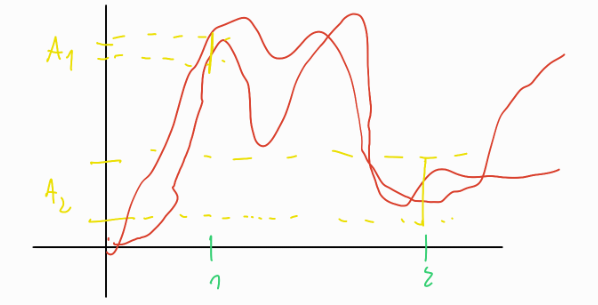
\includegraphics[width=0.7\linewidth]{img/screenshot001}
	\caption{All the functions that are in area 1 at time 1 and in area 2 at time 2 are included in the rectangle}
	\label{fig:screenshot001}
\end{figure}
A random process is a sequence of \rv s but it can also be seen as a one \rv{} measurable on the product space. If $I=[0,\infty)$ then the product space is $\R^{(0,\infty)}$. So we now need to explicitly build a process that is a random process.
\begin{theorem}
	For $t_{1},\ldots,t_{n}\geq0$ with $n\in\N$ and $t_{j}\neq t_{i}$ we assume that 
	\begin{equation*}
		P_{t_{1},\ldots,t_{n}}(\cdot)
	\end{equation*}
	is a family of probability measures for any choice of $n$ and it is on $\left(\R^{n},\B(\R^{n})\right)$.
The Kolmogorov consistency conditions tell us that this family has a random process having this as a distribution. The conditions are:
\begin{enumerate}
	\item $P_{t_{1},\ldots,t_{n}}(A_{1}\times\ldots\times A_{n})=P_{t_{\sigma(1)},\ldots,t_{\sigma(n)}}(A_{\sigma(1)},\ldots,A_{\sigma(n)})$, which means that the distribution is invariant to permutations;
	\item $P_{t_{1},\ldots,t_{n}}(A_{1},\ldots,A_{n-1}\times \R)=P_{t_{1},\ldots,t_{n-1}}(A_{1}\times\ldots\times A_{n-1})$ (integrating the marginal).
\end{enumerate}
If we can specify our family such that $t_{1}<t_{2}<\ldots<t_{n}$ then there exists a unique probability measure $\mu$ on the product space $(\R^{I},\B^{I}(\R))$ such that the canonical process
\begin{equation*}
	X_{t}(\omega)=\omega,\qquad X=\seqtm{X}
\end{equation*}
has finite dimensional distribution $P_{t_{1},\ldots,t_{n}}$. Now take $t_{1}<t_{1}<\ldots<t_{n}$ and 
\begin{equation*}
	T_{t_{1},\ldots,t_{n}}\distnorm{0,\mathbf{C}}
\end{equation*}
with covariance matrix
\begin{equation*}
	\mathbf{C}_{ij}=t_{i}\wedge t_{j}.
\end{equation*}
\end{theorem}

This is just the finite dimensional \bwm{} distribution.
\begin{corollary}
	If $\seqtm{X}$ is a process then there exists a unique measure $\mu$ on the product space such that the canonical process satisfies $X_{0}=0$, then $X_{t}$ has stationary independent and Gaussian increments.
\end{corollary}
Product \sa{} is generated by measurable rectangles, typically by union or intersection; but that is just the combination of a countable number of information and we need to understand what to do when the information is uncountable.
\begin{theorem}
	For every $\Gamma\subset \B^{I}(\R)$ there exists an \textit{at most} countable set $S\subset I$ such that 
	\begin{equation*}
		v\in\Gamma,w\in\R^{I}\;\text{and}\;v|_{S}=w|_{S}\implies w\in\Gamma.
	\end{equation*}
\end{theorem}
This tells us that the product \sa{} is small: for any set in the \sa{} (countably generated) we can find a set of indices which depends on $\Gamma$ and it is countable. If we pick a function  $v$ in $\Gamma$ and we choose another function $w$ in $\B^{I}(\R)$ coinciding with $v$ on $S$ then it must belong to $\Gamma$ as well... but $w$ may be not continuous! This means that the set of continuous functions $C_{0}(I)$ is \underline{not} in $\B^{I}(\R)$. This is an issue because it implies that the set $C_{0}(I)$ is not measurable with respect to the product \sa{} so we cannot compute a probability measure on it.
\end{document} 


%THIS IS THE DARK AGE OF LOVE   $\cdot$